\begin{frame}
	\frametitle{Interaktion Vegetation und Atmosphäre}

		\begin{figure}
		\centering
		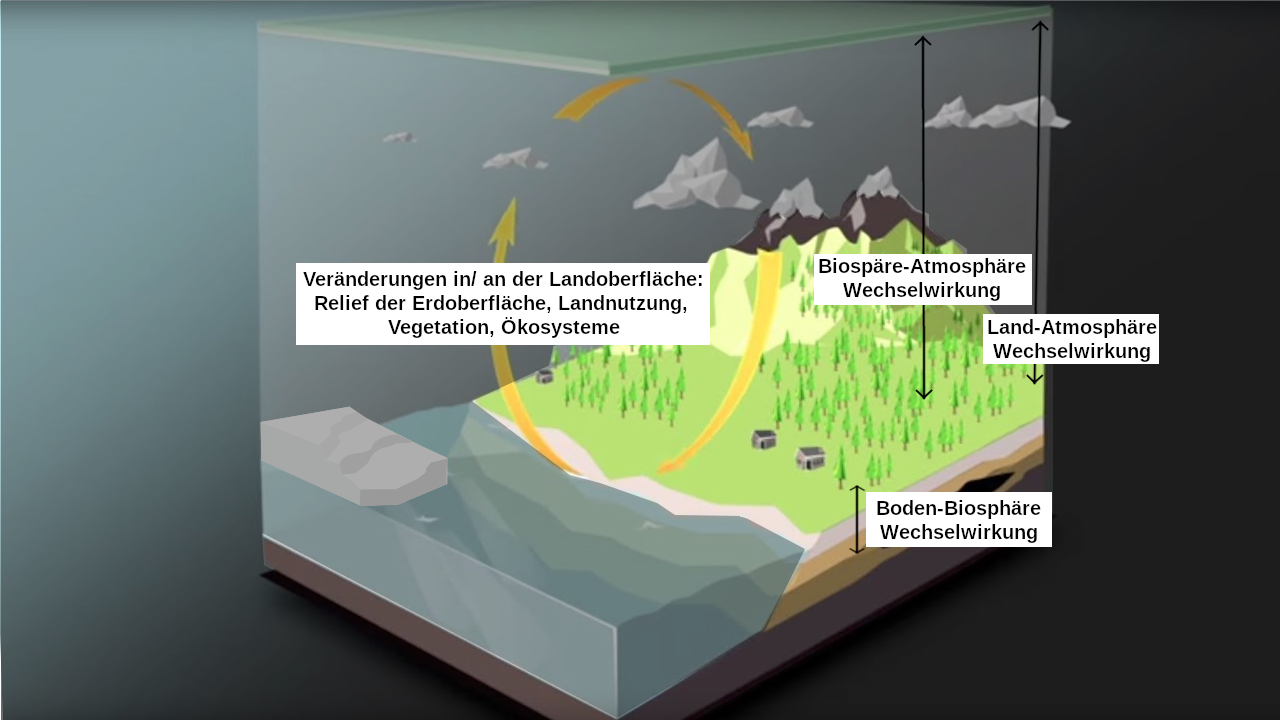
\includegraphics{bilder/WMO_Cycles_factors_landAndGround.png}
		\caption{Interaktion der Biosphäre und Atmosphäre}
	\end{figure}

	\note{
		\begin{itemize}
			\item[] diesmal sind rechts die Wechselwirkungen der Vegetation und Biosphäre zu sehen
			\item[] links sind nochmal die zentralen Elemente der Komponente Vegetation aufgelistet
			\item[] Änderungen an der Landoberfläche durch z.B: Änderung der Landnutzung - Waldrodung, Landwirtschaft...
			\item[] .. ändern auch die Vegetation und die Ökosysteme
		\end{itemize}
	}
\end{frame}
